\documentclass{article}
\usepackage[latin1]{inputenc}
\usepackage[margin=1.0in]{geometry}
\usepackage{fancyhdr}
\usepackage{amsmath}
\usepackage{graphicx}
\usepackage{float}
\usepackage{listings}
\usepackage{color}
\usepackage{caption}
  \usepackage{courier}

\setcounter{secnumdepth}{2}
\setcounter{equation}{0}
\captionsetup{width=10cm}

 \lstset{
         basicstyle=\footnotesize\ttfamily,        % font size for code
         numberstyle=\tiny\color{mygray}, % line number style
         numbersep=5pt,                   % how far the line-numbers are from the code
         tabsize=2,                  % sets default tabsize to 2 spaces (FOR HOWIE :P)
         extendedchars=true,         % non-ascii characters, but not for utf8 enc
         breaklines=true,            % sets automatic line breaking
         keywordstyle=\color{blue},
 	frame=single,                    % adds a frame around the code
         stringstyle=\color{red}\ttfamily, % string literal style
         showstringspaces=false,           % show spaces with underscores
         showtabs=false,             % show tabs within strings adding particular underscores         
         xleftmargin=17pt,
         framexleftmargin=17pt,
         framexrightmargin=5pt,
         framexbottommargin=4pt
 }


\title{Kanto Player \\
CSEE W4840 Final Report}
\author{
  Kavita Jain-Cocks\\
  \texttt{kj2264@columbia.edu}
  \and
  Zhehao Mao\\
  \texttt{zm2169@columbia.edu}
  \and
  Amrita Mazumdar\\
  \texttt{am3210@columbia.edu}
  \and
  Darien Nurse\\
  \texttt{don2102@columbia.edu}
  \and
  Jonathan Yu\\
  \texttt{jy2432@columbia.edu}
   \\}
 \date{\today}
\begin{document}

\maketitle
\newpage

\section{Introduction}
This project presents an audio player with frequency visualization, implemented
on an Altera DE2 Cyclone FPGA. The user is able to play audio files in a custom
encoding from an SD card and view a nice visualization of the audio frequencies
on a VGA display, similar to the visualization on classic music players. Our
implementation uses hardware to handle audio output and frequency
visualization, and software to handle user interaction and system
initialization. The user can interact with the system using switches for color
mixing and buttons for starting and stopping audio playback.

\section{System Architecture}

\subsection{High-Level Overview}

The following is a high-level overview for playing music and displaying 
visualizations using an Altera DE2 Cyclone FPGA.

\begin{figure}[H]
	\centering
	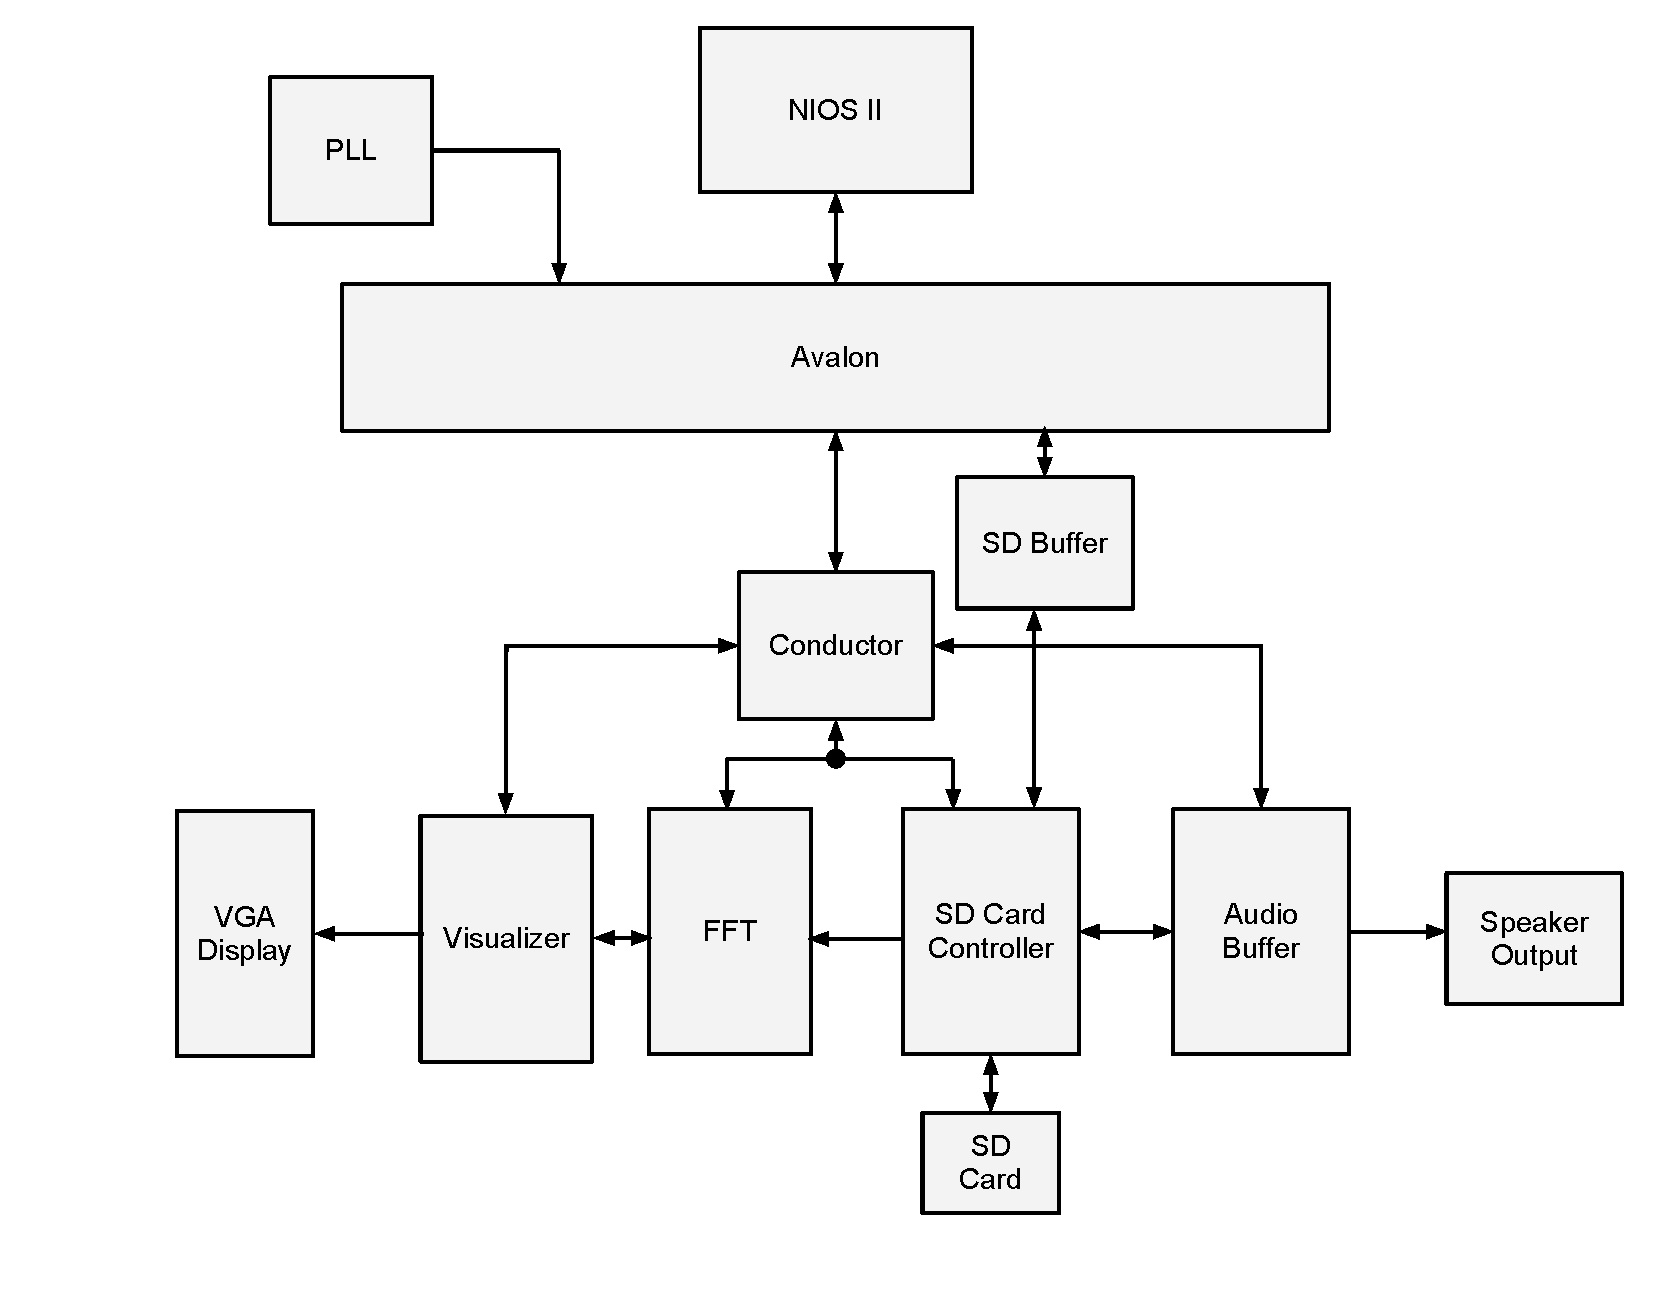
\includegraphics[scale=0.45]{top_level}
	\caption{High-level block diagram of the full \texttt{Kanto} system.}
\end{figure}

\begin{itemize}
	\item Data for the music is stored on the SD card in a time-domain format.
		When the FPGA starts up, \texttt{SD Controller} peripheral performs a 
		series of
		initialization steps to prepare the SD card for processing. Once the 
		SD card is ready, a signal is sent to the \texttt{Conductor} so that some cool 
		stuff can start to unfold.  
	\item The \texttt{Conductor} peripheral, along with the \texttt{NIOS} peripheral,
		controls how and when data flows between every other peripheral. 
		When the \texttt{Conductor} receives the ready signal from the 
		\texttt{SD Controller}, 
		the \texttt{Conductor} transfers control of the system to the \texttt{NIOS} so 
		that 
		software initialization can occur.  
	\item Once the processor gets control, it reads in the first block, which
		is a track table containing the block addresses of each song on the 
		\texttt{SD
		card}. This will allow skipping among tracks. The processor then
		seeks to the first track, reads in the first block of audio data, and
		then returns control to the \texttt{Conductor}.
	\item The \texttt{Audio Buffer} operates on two blocks of memory in the 
		block RAM.
		At any given time, the \texttt{Audio Buffer} is reading data from one block
		while data is being written to the other. The data being read is
		pushed to the audio codec at the audio sampling rate. 
		The next block of data is already written by the time the current audio 
		data is finished being played. The buffer then reads from the newly 
		completed block and new data is written over the old data that was 
		read in the previous block.
	\item The \texttt{FFT} takes the same blocks of data that the \texttt{Audio Buffer} 
		uses
		and performs a 256-point \texttt{FFT}. The \texttt{FFT} converts the time-
		domain data
		to frequency-domain data and stores it in block RAM.  
	\item The \texttt{Visualizer} peripheral is used to display the frequencies
		calculated by the \texttt{FFT} visually. Since humans can only hear
		certain frequencies, the \texttt{Visualizer} isolates and only displays
		the frequencies detectable to the human ear, in this case the
		first 32 frequencies of the 256 calculated by the \texttt{FFT}.  
	\item When the \texttt{Audio Buffer} is done with one block, the 
		\texttt{Conductor} triggers
		the SD card to read in another block. On every fourth block read, the
		\texttt{Conductor }triggers the \texttt{FFT} unit to recompute the frequency 
		values.
		When the \texttt{FFT} unit is done, the conductor triggers the visualizer to
		refresh the display.
\end{itemize}
% include data path
% block diagram
\section{Design Implementation}

\subsection{SD Card Controller}

The SD card controller is responsible for initializing the SD card's own
built-in controller, sending read commands to the SD card as necessary, and
receiving the data and writing it to the audio buffer.  It takes as inputs the
global clock and a 32-bit SD block address to read, and it sends write data,
write address, and write enable to the audio buffer.

\subsubsection{SPI Bus Protocol}

SD cards support three communication protocols: SPI bus mode, 1-bit SD bus
mode, and 4-bit SD bus mode. Our implementation uses the SPI bus, which is the
simplest; the controller acts as the master device, and the SD card acts as a
single slave.  The signals on the SPI bus are:

\begin{itemize}
	\item \texttt{SCLK} - clock, controlled by the master
	\item \texttt{MOSI} - master out, slave in
	\item \texttt{MISO} - master in, slave out
	\item \texttt{CS} - chip select (active low)
\end{itemize}

The controller communicates with the SD card by sending commands over SPI.
The controller must first send a sequence of commands to initialize the SD card.
Once the SD card is initialized and ready, the controller waits for a signal
telling it to perform a read. Once the signal is sent, the controller sends
the read command with the SD card block address as argument and then reads
the response from the SD card.

\begin{figure}[H]
	\centering
	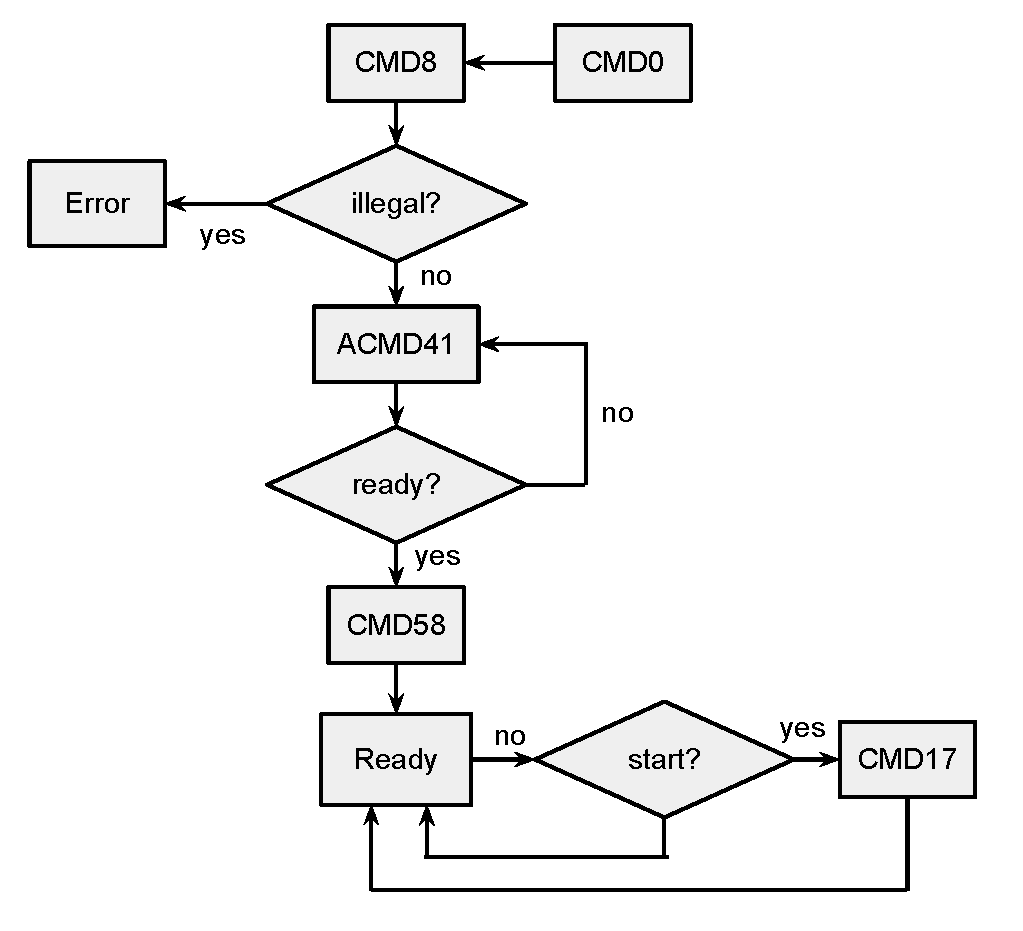
\includegraphics[width=4in]{sd-controller}
	\caption{Flowchart of control signals needed sent by the \texttt{SD Card Controller}. }
\end{figure}

\subsubsection{SD Card Data Formatting}

Support for standard filesystems is not implemented. However, there is support
for multiple song files. SD cards are addressed as 512-byte blocks. As such,
the first 512 bytes of the SD card is dedicated to metadata - it contains the
start addresses for each song on the SD card.

The songs themselves are in 16-bit raw PCM format, written to the SD card end
to end and aligned to 512 byte boundaries. The start addresses of each
song, as discussed earlier, are contained in the metadata block.

\subsection{Audio Buffer}

The audio buffer controls playback of the audio data. It contains a RAM
holding 512 16-bit values and a unit that speaks to the Wolfson WM8731
audio codec on the DE2 board.

\begin{figure}[H]
	\centering
	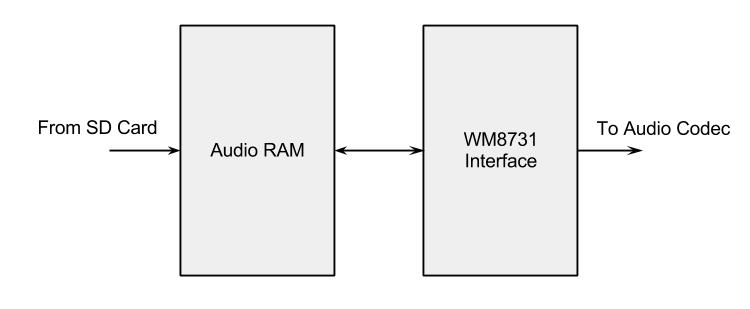
\includegraphics[width=4in]{audio-buffer}
	\caption{High-level block diagram of the \texttt{Audio Buffer} unit.}
\end{figure}

The audio codec interface reads in a 16-bit sample from the audio RAM and
transmits the bits serially to the audio codec. Once the last bit has been
transmitted, the next sample is requested from the audio RAM.

The audio RAM is effectively split in two so that the audio codec interface
plays samples from one half while the SD card writes to the other. This is
the reason why the RAM is chosen to hold 512 samples, since one SD card
block is 512 bytes, or 256 samples. Once the audio codec interface plays 
sample 255 or 511 (indexed from 0), it sends a signal indicating that the 
SD card controller should read in another block.

\subsection{FFT Unit}

The \texttt{FFT} unit is used to compute the discrete frequency transform of a set of 
audio samples to be visualized. 

We use the basic Cooley-Tukey FFT algorithm with a radix of 16 to compute the
frequency transform of a given sample. The number of frequencies \(N\) computed by 
the FFT was chosen to be 256. The radix size and number of frequencies were chosen 
to optimize for space and time. The basic DFT is defined by the equation:

\begin{equation}
	X_k = \sum_{n=0}^{N-1} x_n e^{-\frac{2\pi j}{N} nk}
\end{equation}

The index \(k\) is an integer from 0 to \(N - 1\). Thus, the result of the
transform is a sequence of N complex numbers.

According to the Cooley-Tukey algorithm, we split our original input into 
16 different parts and perform a DFT on each individual component. We can then 
recombine the individual DFT outputs in 4 recombination stages, using the 
following equation for each stage: 

\begin{equation}
	X_k = \left\{
	\begin{matrix}
		E_k + e^{-\frac{2\pi j}{N}k} O_k		& 	\mbox{if } k < N/2 \\ 
		E_{k-N/2} - e^{-\frac{2\pi j}{N} (k-N/2)} O_{k-N/2} & 	\mbox{if }
		k \geq N/2. 
	\end{matrix} 
	\right.
\end{equation}

The FFT hardware consists of two types of pipelines, one for the DFT,
and another for the recombination. 

\begin{figure}[H]
	\centering
	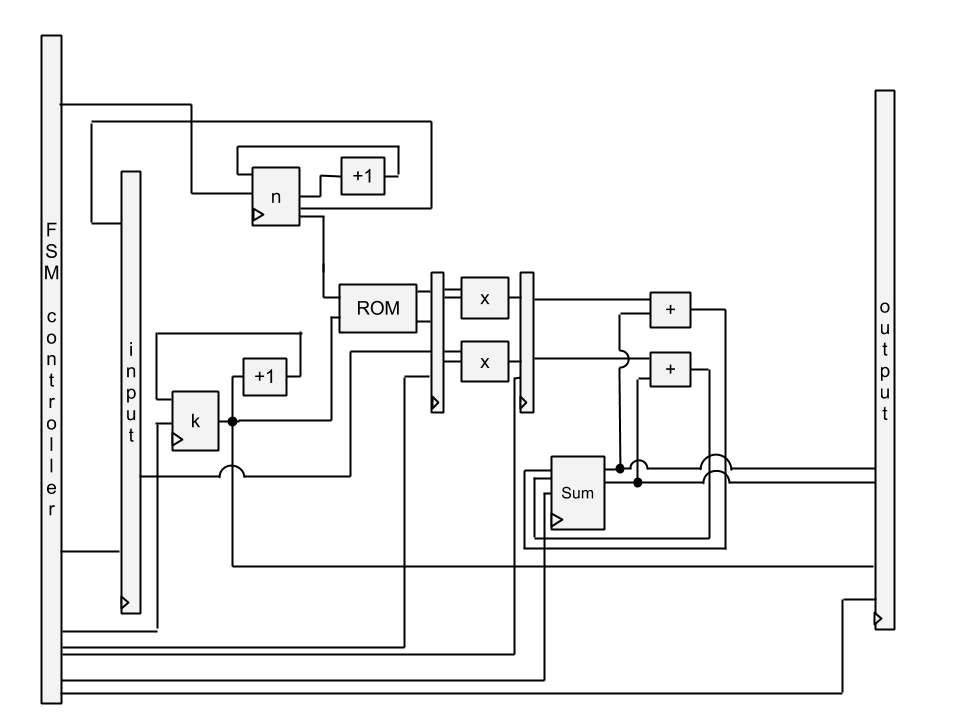
\includegraphics[width=4in]{dft-unit}
	\caption{Block diagram of the \texttt{DFT Unit} pipeline}
\end{figure}

The DFT pipeline computes a 16-point DFT according to equation 1. 

\begin{figure}[H]
	\centering
	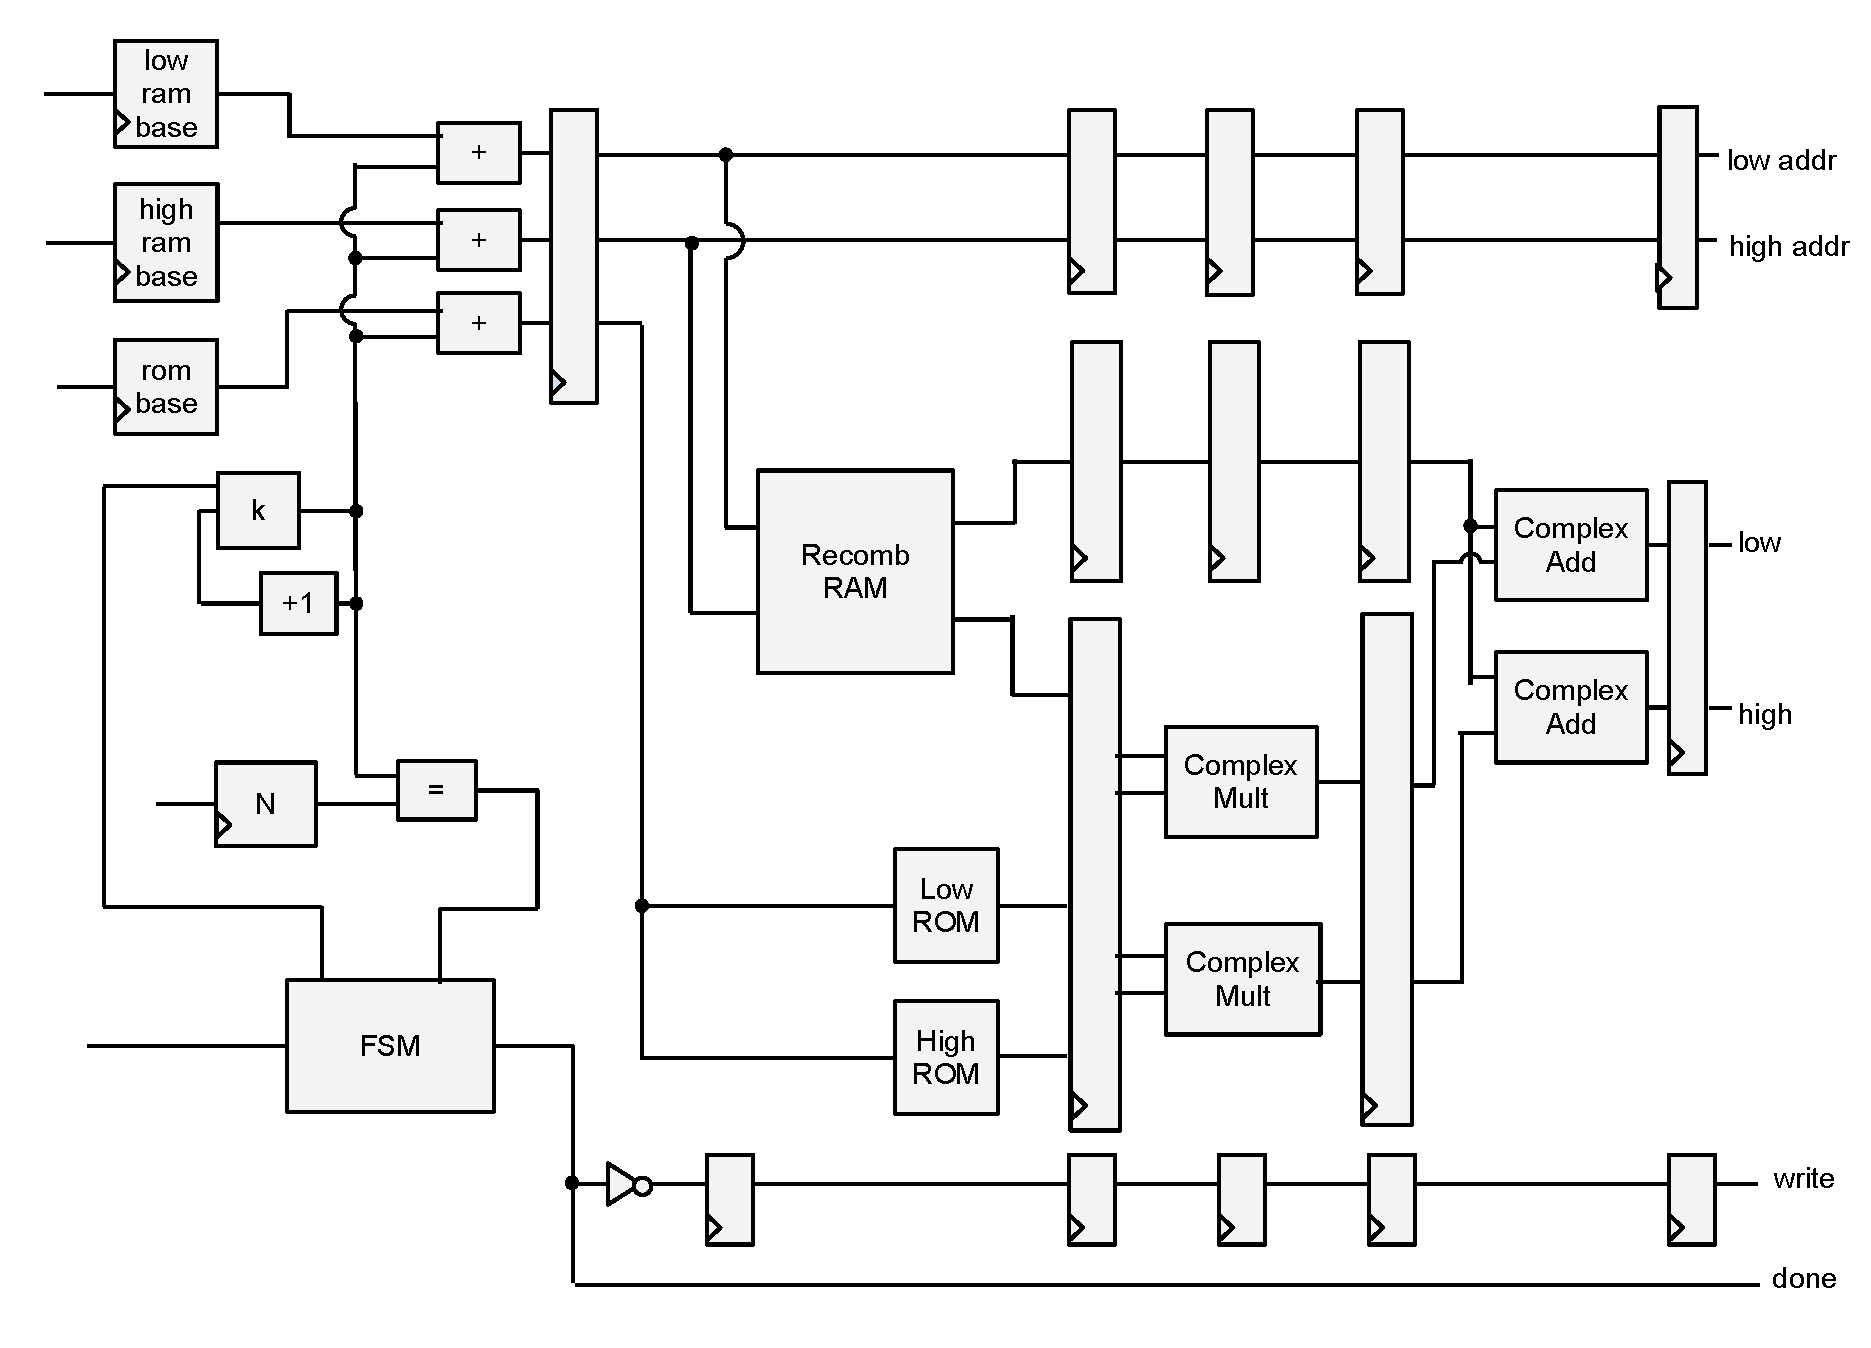
\includegraphics[width=4in]{recombinator}
	\caption{Block diagram of the texttt{Recombination Unit} pipeline}
\end{figure}

The recombination unit computes 32 parts of the recombinational step 
according to equation 2. The upper and lower parts, \(X_k\) and 
\(X_{k + N / 2}\), are computed in parallel. This allows us to re-use the 
odd term \(e^{-\frac{2\pi j}{N}k} O_k\).

The complex multiplier in the recombination unit performs its computation
in two pipelined steps, as follows.

\begin{figure}[H]
	\centering
	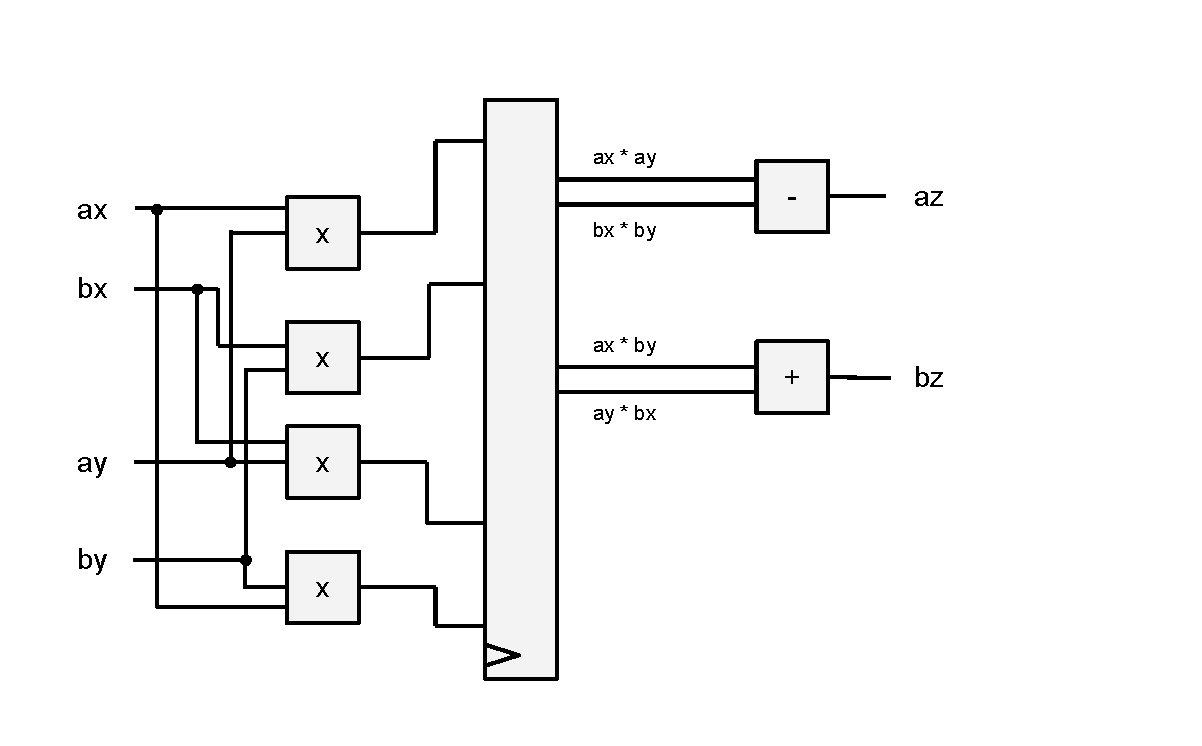
\includegraphics[width=4in]{complex-mult}
	\caption{Block diagram of the \texttt{Complex Multiplier} unit used for 
	recombination. }
\end{figure}

Our top-level FFT block uses two DFT units, a recombination unit,
two RAMs (one for time domain data and one for frequency domain data),
four ROMs for the recombination, one ROM for the DFT coefficients, and
a control unit to set all the multiplexers and control the flow of
computation.

\begin{figure}[H]
	\centering
	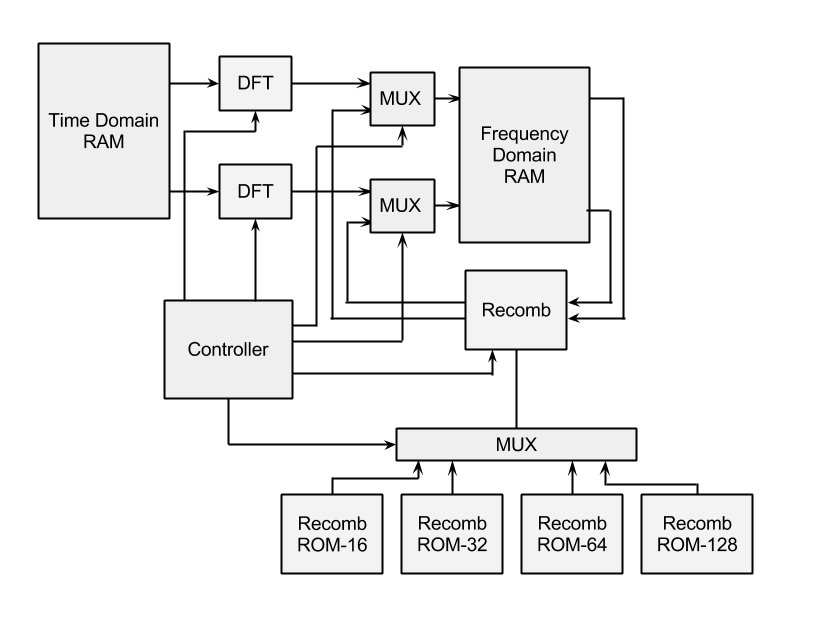
\includegraphics[width=4in]{fft-top}
	\caption{Top-level block diagram of the \texttt{FFT} unit.}
\end{figure}

The DFT ROM holds 256 32-bit values, each one of which represents a
complex number (higher 16 bits for real part and lower 16 bits for
imaginary part). These values represent the constant coefficients
in the DFT equation \(e^{-\frac{2\pi j}{N} n k}\) as 16-bit fixed-point
precision numbers. Each value is addressed by an 8-bit address, where
the highest four bits represent the value of \(k\) and the lowest four bits
represent the value \(n\).

Similarly, the 4 recombination ROMs have 16, 32, 64, or 128 fixed point
imaginary values. These correspond to the constant coefficients
\(e^{-\frac{2\pi j}{N}k}\) from equation 2. The ROMs have 4-bit addresses, 
so only 16 values can be accessed during a single recombination step. 
For the larger ROMs, a select input set by the controller control which 
chunk of 16 values can be addressed.

The controller, in response to an external start signal, triggers
16 DFT computations, with 2 computations running in parallel at a time.
This is followed by 4 stages of recombination. Each recombination stage
uses a different ROM and consists of 8 steps (32 out of 256 outputs are
computed on each step).

The multipliers used in this design all use the dedicated multiplier 
circuitry on the Cyclone II. All RAMs and ROMs use the dual-port M4K
block RAM.
	
\subsection{Visualizer} 

There are two main tasks that the vizualizer needs to accomplish.  
The first is sequentially reading in the data produced by the FFT and the 
other is displaying that data on the vga.  Originally all 256 different 
frequencies were being displayed however after initial designs the decision 
made was to include data for the first 32 frequencies on the display since 
these are the hearable frequencies.  The reading process requires two states, 
a holding state and a reading state.  The transition to reading happens when 
the FFT sends a "done" signal which means that the data is in place to be read.  
For display purposes, the 32 frequencies are placed into 16 bins, 2 per bin, 
each of which corresponds to one of sixteen bars located horizontally across 
the screen.  The height of these bars is decided by summing the amplitude of 
the two frequencies contained in the bin and then scaling this value to the 
necessary height for the screen.

It was necessary to use two different clocks since the VGA display requires a 25.1 MHz clock, in this case a 25 MHz clock as used.  There was no need to read in data on the slower clock and therefore the a 50 MHz clock was used there so as to read the data as quickly as possible. 

An additional functionality that was added was the ability to change color of the bars appearing on the screen.  
Three switches correspond to red, green, and blue and allow the user to mix 
and match to create different colors.  The switches are active low so the 
default color when all switches are "off" is the white so as to be seen on the 
black background.  In order to improve the accuracy of the display adjustments 
were made so that new data is only read in when data is not being drawn to the screen.

\begin{figure}[H]
	\centering
	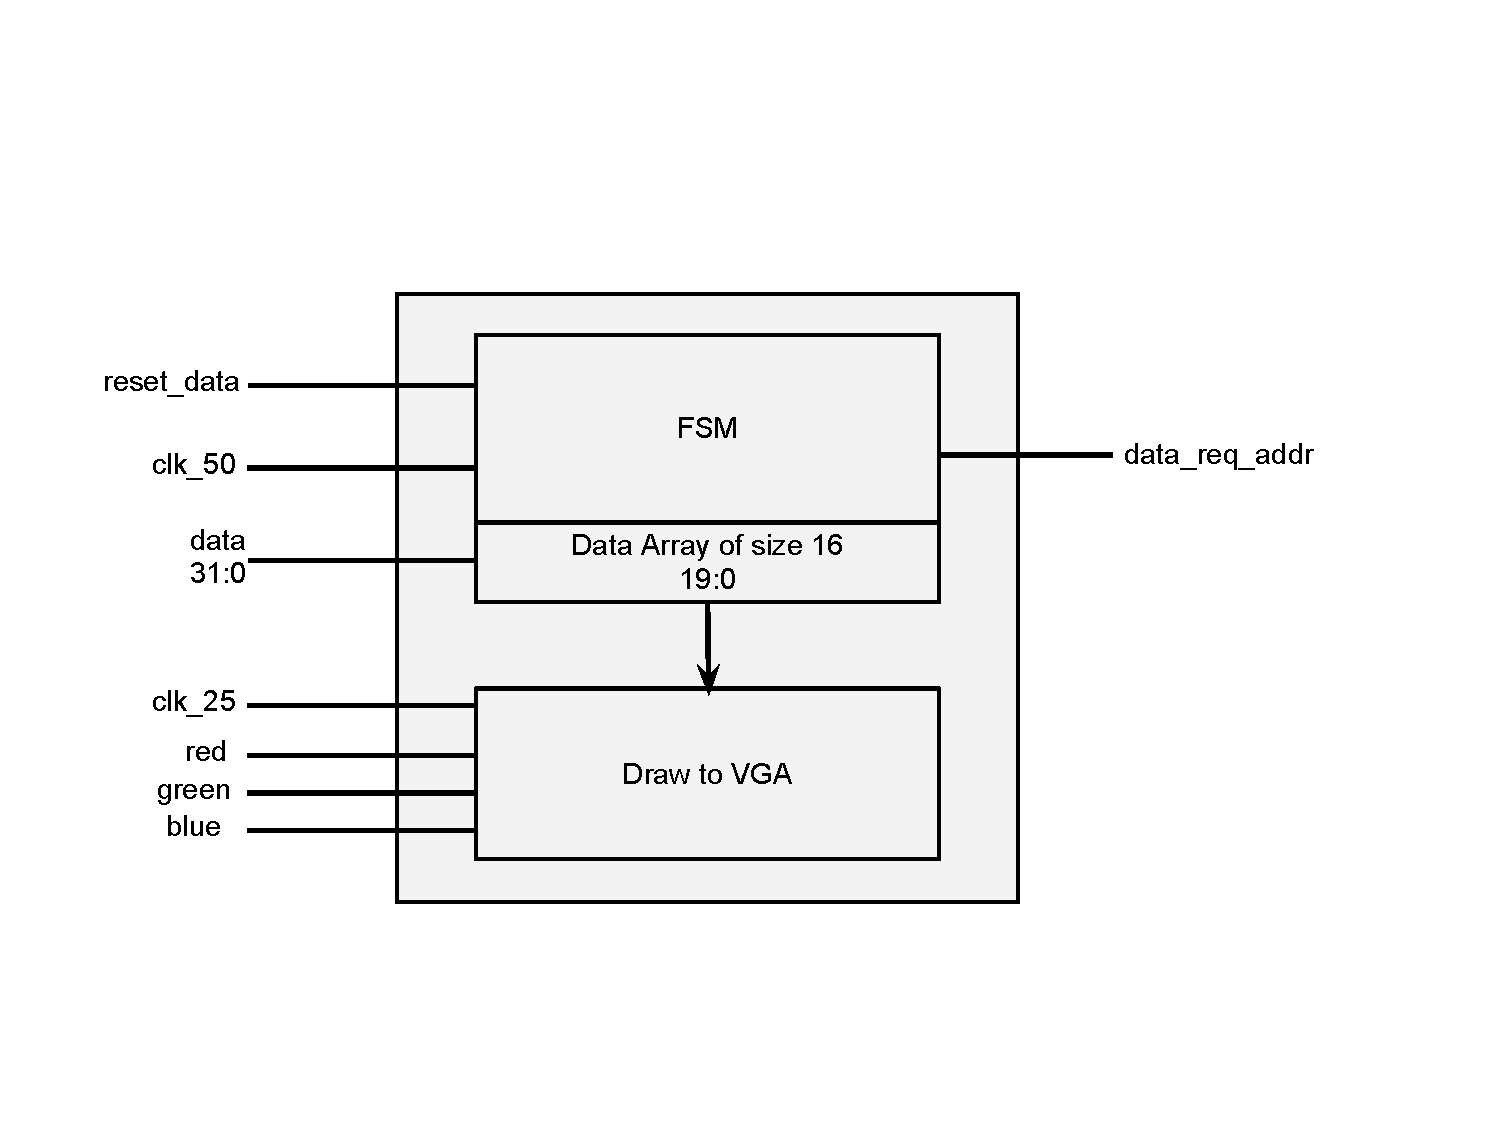
\includegraphics[width=4in]{viz_block_diagram}
	\caption{Block diagram of \texttt{Visualizer} unit.}
\end{figure}

\subsection{Software User Interface}

This project was initially created using only hardware components. The NIOS 
entity was added later in order to give the project additional functionality. 
At startup, the software reads in the first block of data from the SD card. 
This first block contains 32-bit numbers which are the block addresses of the 
beginning of each song on the SD card. If there are fewer than 128 songs on the 
SD card, the remaining words in the block will be set to 0. The last non-zero 
word in the track table is the end of the last track. Once intialization is
finished, the NIOS software hands control over the system to the hardware
conductor. It then goes into a loop in which it polls the current block address
and the state of the push buttons. If the current block address goes over the 
first block address of the next track, the track number is updated internally
as well as written to a set of seven-segment displays. If one of the track 
switch buttons is pressed, the program takes control away from the conductor,
changes the block address to the start of the new track, reads in that block,
and then returns control to the conductor.
\begin{figure}[H]
  \centering
    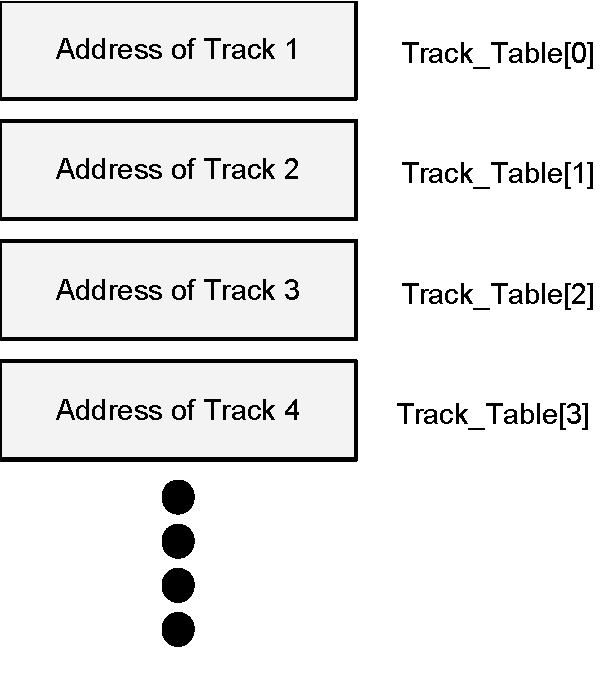
\includegraphics[width=2in]{track_table_diagram}
  \caption{Visual representation of the track table created by the \texttt{NIOS} 
component.}
\end{figure}

\subsection{Miscellaneous Controller Components}
\subsubsection{The Conductor}
The conductor unit handles system coordination and communication between modules, and is the primary controller unit for the system. Typical system operation and data flow within the module is as follows:
\begin{itemize}
	\item \texttt{initial} --- When the system starts up, the conductor begins 
		in the \texttt{initial} state. It waits for the SD card to finish 
		intialization (sd\_ready is high) and then hands off control to the NIOS 
		system for system initialization and playback control in the 
		\texttt{cpuctrl} state.
	\item \texttt{cpuctrl} --- In this state, the NIOS system is handling user 
		interaction. If the signal \texttt{nios\_readblock} is high, the 
		conductor will trigger read of a single block of data from the SD card
		by entering the trigger\_write state. Otherwise, if the \texttt{nios\_play} 
		signal is high, the system can begin or resume audio playback by 
		transistioning into the resume state. In this condition, the block 
		address to be read from is incremented.
	\item \texttt{trigger\_write} --- This state is a transitional state to set
		sd\_start high for one clock cycle. The conductor immediately 
		transistions from this state to wait\_write
	\item \texttt{wait\_write} --- In this state, the module waits until the 
		\texttt{sd\_ready} flag is set high, indicating that a block has been 
		read and control can be returned to the CPU.
	\item \texttt{resume} --- This state resets the \texttt{fft\_counter} 
		signal to 0 before audio playback begins.
	\item \texttt{playing} --- This state is the default state when playback
		is occurring. Depending on the status signals, the conductor could
		switch into block\_end or fft\_end. If nios\_play is set low, the
		conductor switches to the \texttt{initial} state to return the SD card 
		to CPU control.
	\item \texttt{block\_end} --- The conductor enters this state for one
		clock cycle after the audio buffer switches buffers. It triggers a 
		read from the SD card and, on every fourth block, triggers the FFT.
		The conductor also increments the SD card block address.
	\item \texttt{fft\_end} --- The conductor enters this state when the FFT
		unit finishes computing (fft\_done changes from low to high). In this
		state, the visualizer reset is triggered.
\end{itemize}
\begin{figure}[H]
  \centering
    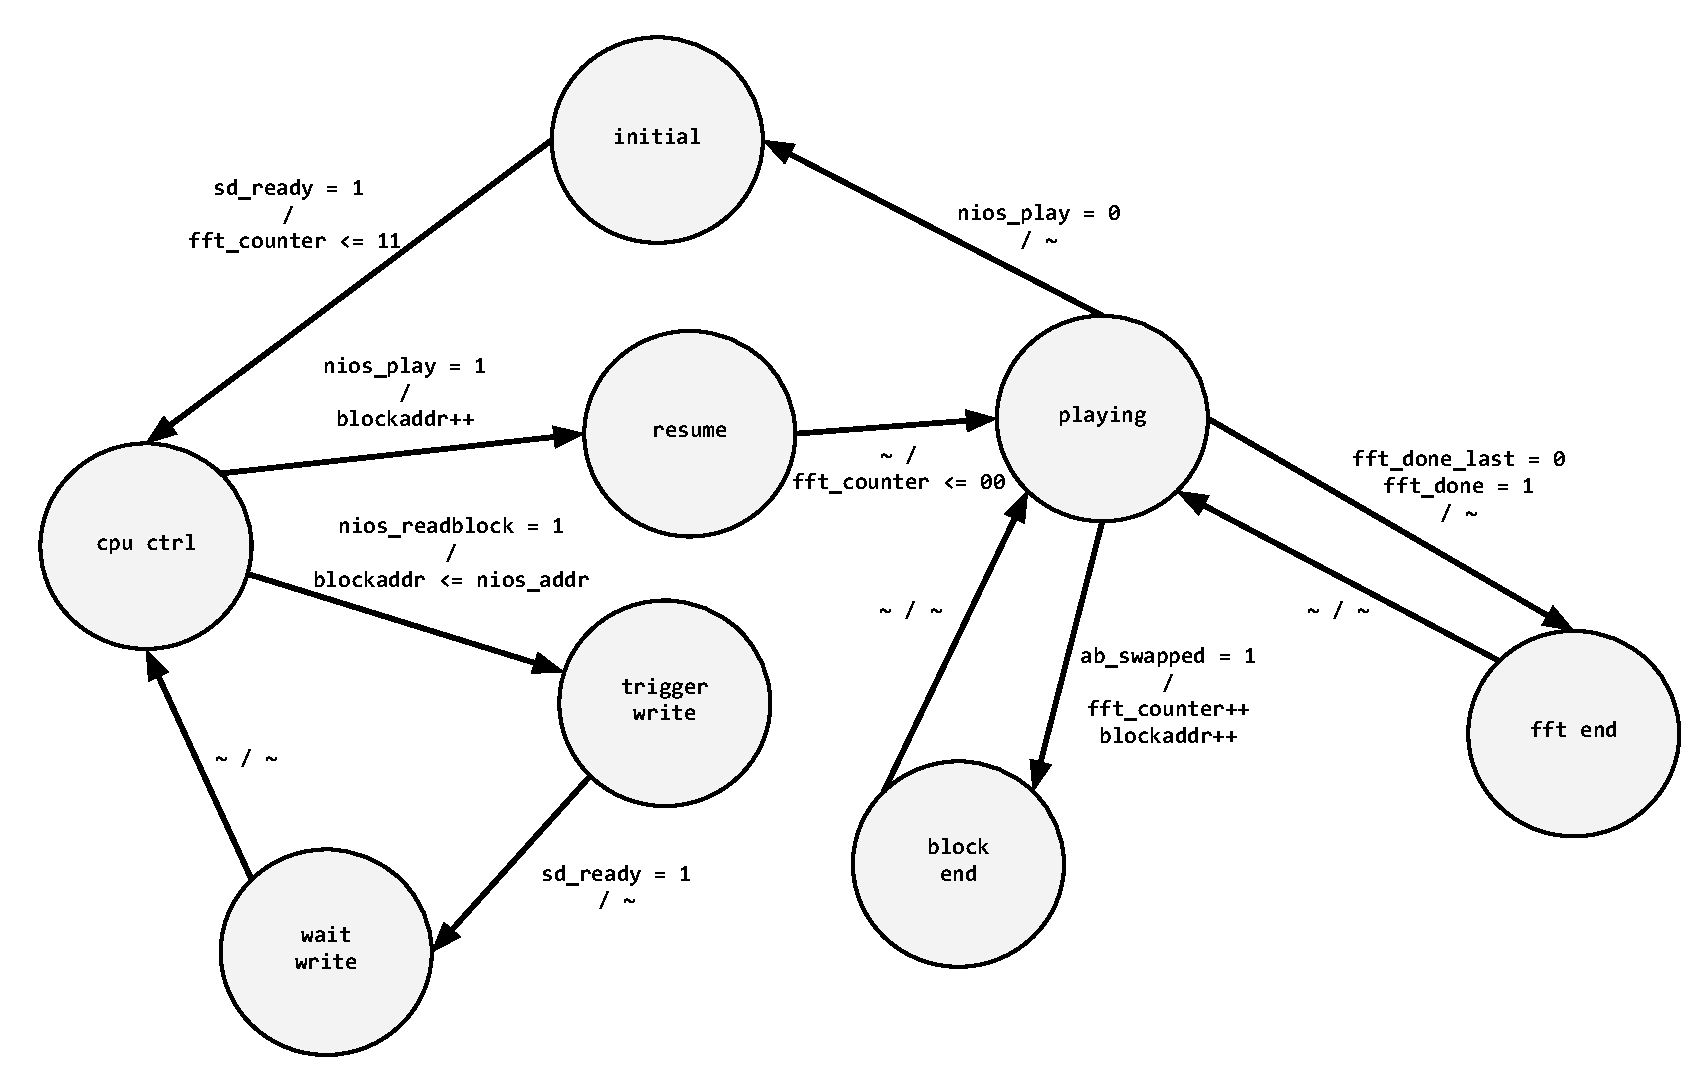
\includegraphics[width=6in]{conductor_state}
  \caption{Simplified State Diagram for the \texttt{Conductor} unit:
    Mealy machine, using abstract transition descriptions and omitting unused
    signals for compactness. \(\widetilde{}\)   denotes a lack of outputs}
\end{figure}
\subsubsection{Phase-Locked Loop for Multiple Clocks}
The visualizer unit and audio playback required different clocks to drive their respective peripherals, but also required clocks to synchronize communication with other modules in the kanto system. To most easily configure these clocks, a Phase-Locked Loop (PLL) was generated from an Altera Megafunction. The PLL was used to generate a 50MHz clock for general system synchronization, a 25MHz clock to drive the VGA display, and an 11.29MHz clock for the audio output.

\section{Design Changes}
\subsection{Removal of SRAM}

In our initial design, we planned on using the SRAM to store the values for the audio 
buffer and the output of the FFT unit. Separate components would communicate by 
reading and writing values to the SRAM. We had implemented an SRAM controller 
with four-phase handshaking to multiplex among the different components. We 
eventually found, however, that our memory usage did not justify the extra complexity 
that using SRAM imposed on our design, so we ended up using on-chip block RAM 
instead.

\subsection{Adding Software Control}

Initially, our design was implemented entirely in hardware, as we found our control 
scheme wasn�t complex enough to require software. However, in order to satisfy the 
requirements for the class, we had to add a software component. We decided to use 
software to coordinate the initialization of our system, as well as track switching, and 
have the hardware controller (the conductor) take over when the audio is actually 
playing. 

\subsection{Display Changes}

After connecting the FFT and visualizer units together, we determined the visualizer 
would be more aesthetically pleasing if we isolated and displayed only the 
frequencies detectable to the human ear, in this case the first 32 frequencies of the 
256 calculated by the FFT.  Another aesthetic change made was to provide the user 
with the capability of changing the color of the visualization.

\section{Testing Methodology}

Testing proved to be helpful in isolating and fixing bugs before introducing
modules into the system. For computational units and controllers, testing was
done through simulations and assertions; for peripherals, testing was done by
using test drivers and observing the peripherals behavior. The following
sections provide a brief overview of our testing procedures for major
components.

\subsection{FFT Controller}

The FFT algorithm was implemented in C early on. A sample input was run through
the software FFT to generate a corresponding output, and we tested by comparing
this output to the output generated in hardware given the same input. As we
modified the FFT (for instance, to reduce parallelism and use block ram), we
continually tested against this sample to make sure the hardware was still
mathematically correct.

\subsection{Visualizer}

The two major tests of correctness for the visualizer were 1) displaying each
of the bars at the correct height; and 2) quickly refreshing the screen when
the registers were updated. To test this, we wrote a hardware driver that set
the bars at two different levels and flipped back and forth between them while
we observed the changes on the VGA monitor.

\subsection{Audio Buffer}

The audio buffer needed to produce a clean sound with no crackling. This tested
by writing in a sine wave and listening to the output. Additionally, a
simulation testbench was used to ensure that swapping between the two buffers
was properly synchronized.

\subsection{SD Card Controller}

We tested the SD card controller by block level writing known data onto an SD
card and ensuring that the same data was read back. Because there are numerous
intermediate steps in communicating with an SD card, various LEDs and 7-segment
displays indicate the current state of the state machine, allowing us to see
where commands have failed.

\subsection{Conductor}

The conductor is the glue that holds all the components together. We emulated
the system components in a testbench and simulated the signals they would
output; using assertions, we confirmed that the conductor was correctly timing
the interactions between components.

\section{Timeline \& Milestone Progress}
\begin{tabular}{cc|p{7cm}p{3cm}}
\textbf{Milestone} & \textbf{Date} & \textbf{Goal} & \textbf{Accomplished}\\ \hline
&&&\\
Milestone 1 & Apr 2 & RTL design and block diagrams of all peripherals.&
	\textit{Completed.}\\
&&&\\
Milestone 2 & Apr 16 & Individual peripherals written in VHDL and test benched.&
	\textit{Completed.}\\
&&&\\
Milestone 3 & Apr 30 & Build interfaces between all peripherals and finish synchronization software. &
	\textit{Completed}\\
&&&\\
Deadline&May 15&System complete and presentation finished.&\textit{Completed.}\\
&&&\\
\end{tabular}
%% should include software inclusion somewhere


\section{Distribution of Work}
\begin{itemize}

\item
	\textbf{Kavita Jain-Cocks}
	\begin{enumerate}
		\item Visualizer
		\item SD Controller
	\end{enumerate}

\item 
	\textbf{Zhehao Mao}
	\begin{enumerate}
		\item FFT
		\item Audio Buffer
		\item SD Controller
		\item Conductor
		\item Software
	\end{enumerate}

\item 
	\textbf{Amrita Mazumdar}
	\begin{enumerate}
		\item Visualizer
		\item FFT
	\end{enumerate}

\item 
	\textbf{Darien Nurse}
	\begin{enumerate}
		\item Visualizer
		\item Software
	\end{enumerate}

\item 
	\textbf{Jonathan Yu}
	\begin{enumerate}
		\item SD Controller
		\item Software
	\end{enumerate}

\end{itemize}

\section{Challenges \& Lessons Learned}

\subsection{Interfacing to External Hardware}

Interfacing to external hardware like the SD card and the audio codec were by far the 
most challenging parts of the assignment, mainly because they were difficult to 
debug. Since proper functionality depended on what the external hardware was 
doing, we couldn't reliably use Quartus testbenches like we did for the rest of the 
components, since our testbenches wouldn't exactly replicate the behavior of the 
external hardware. We found that the best way to get interfaces to external hardware 
working was to base our implementation off of successful existing implementations. 
For instance, for the audio buffer, we used the components provided for Lab 3 to 
interface with the audio codec, but modified the files to achieve the correct sampling 
frequency. For the SD card controller, we based a lot of our code off of the SPI 
controller from Prof. Edward's Apple II FPGA project, as well as the SD card driver 
code in the Linux Kernel. 

\subsection{Changing Parallelism Levels}

Because of the extensive parallelism in the FFT module, it became difficult to fit the 
entire system on the FPGA, and we had to reduce the amount of parallelism in the 
FFT unit to decrease the number of logic gates used by the board. We found that 
reducing the level of parallelism is often just as hard, if not harder, than adding 
parallelism, and that both actions require extensive changes to the design of a 
system. It would have made things much easier if we had decided on the proper level 
of parallelism at the outset. If we had done some quick calculations at the outset, we 
would have discovered that could have used a very low level of parallelism and still 
been well within the deadlines imposed by the timing of our system.

\subsection{Timing Issues}

Timing issues can be a big problem in a complex design, especially if external 
hardware is involved, as different hardware peripherals require different clocks. For 
our design, the audio codec used a 11.29 MHz clock, the VGA used a 25 MHz clock, 
and the SD card used a 6.25 MHz clock. We used a PLL for the first two and clock 
enables for the last one (since the SD card clock wasn�t always running). But passing 
status and control signals between units running on different clocks ended up being a 
minor challenge as well. We ended up solving this problem by either stretching the 
signals or detecting the rising edge of signals. 

Because the operations of reading in VGA data and refreshing the VGA display both 
took more than one cycle meant that we needed to ensure that the data wasn�t being 
changed while the display was in the middle of refreshing. This was accomplished by 
reading data into a separate set of registers and only transferring it to the registers 
used by the display processes once the refresh had reached the edge of the screen.  
This made it possible to reduce flickering that was being seen on the display.

\subsection{Reduction of Hardware Usage}

At its peak, our design used up 89\% of the logic elements on the FPGA. We found out 
that this was because we were accidentally using logic elements instead of block 
RAM for all of our memory components. After switching over the memory components 
to block RAM, our logic element usage went down to only 10\%, while our block RAM 
usage went from 1\% to only 5\%. This showed us the importance of actually using 
memory elements for memory.

Shifting our memory components to block RAM did require a lot of other changes to 
our design. For instance, since the block RAM only had two ports, we had to 
dramatically reduce the amount of parallelism in the FFT unit. We also had to 
duplicate some memory. For instance, the FFT unit and audio buffer initially shared 
the same memory for the time domain samples, but we eventually separated this into 
two different RAMs which the SD card controller wrote to simultaneously. Although 
these practices seemed counterintuitive, this duplication did not add that much to our 
memory requirements, as noted above. 

Having a modular design, both at the highest level and at the level of each
component, made these changes go relatively smoothly.

\section{Reflections \& Prospectus}

Our group is very satisfied with the final version of our project. We accomplished all 
major project goals, and added improved functionality in certain modules, such as 
color changes in the visualizer and track selection. Although certain elements did not 
conform to the originally-delineated system design, such as replacing the SRAM with 
block RAM and changing the role of software in the high-level design, we feel the 
project exceeds our original goals for the project. There were a few areas under 
which our group could have improved, namely in scheduling and deliverables, and 
further design optimizations.

\subsection{Scheduling \& Deliverables}
Because of the modular nature of our system design, our plan for project completion 
involved developing and optimizing each component fully in isolation, and then 
linking them together afterwards. Although this plan was successful for our group, a 
more productive strategy could have been a more sequential approach to system 
design, starting with critical components, such as the SD card, and moving linearly 
through the different components, ending with the visualizer.  This method would 
have allowed us to have more concrete deliverables during milestones and helped 
us detect system-wide issues earlier on, such as the heavy use of logical elements in 
our memory and FFT designs. 

Another consequence of our scheduling was that, although we remained fairly on 
track with our predetermined milestones and ended up completing the design ahead 
of schedule, our description of milestones and deliverables was extremely vague and 
hard to verify during the biweekly milestone check-ins. This could have been 
remedied in multiple ways. One option would have been to choose more specific, 
tangible deliverables at each milestone to demonstrate our progress. Another would 
have been to review our milestones with Professor Edwards or our adviser before 
deciding upon them. 

One situation that needed to be contended with was that we had a larger group size 
to begin with and also lost a group member early in the process. The large group size 
was challenging because we needed to ensure the project goals were split evenly 
and progress was continuously being made, while grappling with the schedules of 
many different team members. Losing a group member only compounded the 
problem, because we had to reorganize some of the work distribution early on in the 
initial design phase. To address this, our team worked hard to maintain continued 
lines of communication via e-mail checkups and twice-weekly meetings. We felt that 
by staying organized and updating the entire group regularly on our progress, we 
were able to stay informed about the status of the project and what our immediate 
next tasks were, as well as reorganize tasks to compensate for the lost group 
member. Some invaluable tools used for group management were \texttt{Google 
Groups} and \texttt{Google Drive} for group email and documentation organization, 
and \texttt{Github Organizations} to manage our repositories of project code.

\subsection{Optimizations \& Improvements}

Although all the initial project goals have been accomplished, there are always 
more improvements and new features that could be implemented.
For instance, the visualization could be made more complex than simply 
displaying bars for each frequency. Having a more interesting visualization 
would vastly improve the "coolness" factor of our project. Another possible 
improvement would be to change the SD card format from our custom format to a 
standard FAT filesystem. This would make it easier for the user to add songs to 
the SD card, as they could simply copy audio files to the filesystem instead of 
having to use custom tools for converting the data and writing it to the block 
device.

\newpage
\appendix

\section{Source Code}
\subsection{VHDL}
	\subsubsection{kanto.vhd}
	\lstinputlisting[language=VHDL]{../kanto/kanto.vhd}
	\subsubsection{audio\_buffer.vhd}
	\lstinputlisting[language=VHDL]{../kanto/audio_buffer.vhd}
	\subsubsection{complex\_mult.vhd}
	\lstinputlisting[language=VHDL]{../kanto/complex_mult.vhd}
	\subsubsection{conductor.vhd}
	\lstinputlisting[language=VHDL]{../kanto/conductor.vhd}
	\subsubsection{de2\_kanto\_ctrl.vhd}
	\lstinputlisting[language=VHDL]{../kanto/de2_kanto_ctrl.vhd}
	\subsubsection{de2\_sd\_buffer.vhd}
	\lstinputlisting[language=VHDL]{../kanto/de2_sd_buffer.vhd}
	\subsubsection{de2\_sram\_controller.vhd}
	\lstinputlisting[language=VHDL]{../kanto/de2_sram_controller.vhd}
	\subsubsection{de2\_wm8731\_audio.vhd}
	\lstinputlisting[language=VHDL]{../kanto/de2_wm8731_audio.vhd}
	\subsubsection{dft\_stage1.vhd}
	\lstinputlisting[language=VHDL]{../kanto/dft_stage1.vhd}
	\subsubsection{dft\_stage2.vhd}
	\lstinputlisting[language=VHDL]{../kanto/dft_stage2.vhd}
	\subsubsection{dft\_stage3.vhd}
	\lstinputlisting[language=VHDL]{../kanto/dft_stage3.vhd}
	\subsubsection{dft\_tb.vhd}
	\lstinputlisting[language=VHDL]{../kanto/dft_tb.vhd}
	\subsubsection{dft\_top.vhd}
	\lstinputlisting[language=VHDL]{../kanto/dft_top.vhd}
	\subsubsection{fft\_controller.vhd}
	\lstinputlisting[language=VHDL]{../kanto/fft_controller.vhd}
	\subsubsection{fft\_tb.vhd}
	\lstinputlisting[language=VHDL]{../kanto/fft_tb.vhd}
	\subsubsection{fft\_fdom\_ram.vhd}
	\lstinputlisting[language=VHDL]{../kanto/fft_fdom_ram.vhd}
	\subsubsection{fft\_recomb.vhd}
	\lstinputlisting[language=VHDL]{../kanto/fft_recomb.vhd}
	\subsubsection{fft\_tdom\_ram.vhd}
	\lstinputlisting[language=VHDL]{../kanto/fft_tdom_ram.vhd}
	\subsubsection{recomb\_stage1.vhd}
	\lstinputlisting[language=VHDL]{../kanto/recomb_stage1.vhd}
	\subsubsection{recomb\_stage2.vhd}
	\lstinputlisting[language=VHDL]{../kanto/recomb_stage2.vhd}
	\subsubsection{recomb\_stage3.vhd}
	\lstinputlisting[language=VHDL]{../kanto/recomb_stage3.vhd}
	\subsubsection{recomb\_tb.vhd}
	\lstinputlisting[language=VHDL]{../kanto/recomb_tb.vhd}
	\subsubsection{sd\_controller.vhd}
	\lstinputlisting[language=VHDL]{../kanto/sd_controller.vhd}
	\subsubsection{sdbuf.vhd}
	\lstinputlisting[language=VHDL]{../kanto/sdbuf.vhd}
	\subsubsection{sevenseg.vhd}
	\lstinputlisting[language=VHDL]{../kanto/sevenseg.vhd}
	\subsubsection{visualizer.vhd}
	\lstinputlisting[language=VHDL]{../kanto/visualizer.vhd}

\subsection{Verilog}
	\subsubsection{de2\_i2c\_av\_config.v}
	\lstinputlisting[language=Verilog]{../kanto/de2_i2c_av_config.v}
	\subsubsection{de2\_i2c\_controller.v}
	\lstinputlisting[language=Verilog]{../kanto/de2_i2c_controller.v}

\subsection{C}
	\subsubsection{main.c}
	\lstinputlisting[language=C]{../kanto/software/kanto_software/main.c}
	\subsubsection{fft/comp2real.c}
	\lstinputlisting[language=C]{../kanto_tools/fft/comp2real.c}
	\subsubsection{fft/dftcoeffgen.c}
	\lstinputlisting[language=C]{../kanto_tools/fft/dftcoeffgen.c}
	\subsubsection{fft/dftsim.c}
	\lstinputlisting[language=C]{../kanto_tools/fft/dftsim.c}
	\subsubsection{fft/rccoeffgen.c}
	\lstinputlisting[language=C]{../kanto_tools/fft/rccoeffgen.c}
	\subsubsection{fft/recombsim.c}
	\lstinputlisting[language=C]{../kanto_tools/fft/recombsim.c}
	\subsubsection{fft/sumbins.c}
	\lstinputlisting[language=C]{../kanto_tools/fft/sumbins.c}
	\subsubsection{sdcard/crc7\_calc.c}
	\lstinputlisting[language=C]{../kanto_tools/sdcard/crc7_calc.c}
	\subsubsection{sdcard/pcm2text.c}
	\lstinputlisting[language=C]{../kanto_tools/sdcard/pcm2text.c}
	\subsubsection{sdcard/testdata.c}
	\lstinputlisting[language=C]{../kanto_tools/sdcard/testdata.c}
	\subsubsection{sdcard/text2pcm.c}
	\lstinputlisting[language=C]{../kanto_tools/sdcard/text2pcm.c}

\subsection{Python} %should we include python scripts to generate things? eh
	\subsubsection{fft/inputgen.py}
	\lstinputlisting[language=Python]{../kanto_tools/fft/inputgen.py}
	\subsubsection{fft/plot.py}
	\lstinputlisting[language=Python]{../kanto_tools/fft/plot.py}
	\subsubsection{roms/arraygen.py}
	\lstinputlisting[language=Python]{../kanto_tools/roms/arraygen.py}
	\subsubsection{roms/mifgen.py}
	\lstinputlisting[language=Python]{../kanto_tools/roms/mifgen.py}
	\subsubsection{sdcard/mkauimg.py}
	\lstinputlisting[language=Python]{../kanto_tools/sdcard/mkauimg.py}

\subsection{Shell}
	\subsubsection{fft/fftsim.sh}
	\lstinputlisting[language=Bash]{../kanto_tools/fft/fftsim.sh}
	\subsubsection{sdcard/playimage.sh}
	\lstinputlisting[language=Bash]{../kanto_tools/sdcard/playimage.sh}
 
\end{document}
